In order to test the validity of using neural networks trained
on molecular dynamics trajectories to generate new trajectories
we train neural networks on systems of copper and silicon atoms
using the Effective Medium Theory \cite{jacobsen1996semi}
and Stillinger-Weber \cite{che8002013} potentials
respectively.
These potentials have efficient implementations
through the Atomic Simulation Environment (ASE)
and their As Soon As Possible (ASAP) interface, which makes
it ideal for our purposes. Additionally these potentials
have an intermediate complexity, with Stillinger-Weber explicitly
including three-body interactions, which makes them ideal
for testing whether the Behler-Parrinello method \cite{behler2007generalized}
can replicate this.
At temperatures which are not too large these potentials describe
atoms in a crystalline structure in equilibrium,
and we test whether the neural network can reproduce the correct potential
energy, forces, radial distribution and mean squared displacement.
In table \ref{tab:hyperparam} we have listed the parameters we have
used in the training process. While we have used a large amount
of training images for the energy training, since this is relatively
inexpensive, 8000 training images were not a noticeable improvement
over approximately 5000-1000 images,
and only seemed to affect the speed of convergence.
We finally used 1000 images to refine the force accuracy,
as we discussed in the previous chapter.
In table \ref{tab:hyperparam-test} we have listed the parameters
used for testing the neural network. For sampling data we used a larger
timestep and sampling interval
than for applying the neural network, in order to obtain
a larger diversity of configurations, though this did not appear to
matter much in the final analysis.

% Mention loss vs RMSE here...?

\begin{table}[H]
\centering
\caption{Hyperparameters used in fitting the neural network
    to the copper and silicon images.}
\label{tab:hyperparam}
\begin{tabular}{|c c|}
\hline
Hyperparameter & Value \\
\hline \hline
    Hidden layers & $\left[10, 10\right]$ \\
Activation & Hyperbolic tangent \\
    Time (fs) & $9 \cdot 10^5$ \\
    Timestep (fs) & 5 \\
    Sampling intervall (timesteps) & 100 \\
Max epochs & 4000 \\
    Regularization & $\lambda = 10^{-7}$ \\
Optimizer & BFGS \\
Energy coefficient & 1.0 \\
Force coefficient & 0.1 \\
\hline
\end{tabular}
\end{table}

\begin{table}[H]
\centering
\caption{Hyperparameters used in testing the trained copper and
    silicon neural networks.}
\label{tab:hyperparam-test}
\begin{tabular}{|c c|}
\hline
Hyperparameter & Value \\
\hline \hline
    Hidden layers & $\left[10, 10\right]$ \\
Activation & Hyperbolic tangent \\
    Time (fs) & $5 \cdot 10^3$ \\
    Timestep (fs) & 1 \\
    Sampling intervall (timesteps) & 10 \\
\hline
\end{tabular}
\end{table}

\subsection{Effective Medium Theory}\label{chap:emt}
The Effective Medium Theory (EMT) potential 
\cite{jacobsen1987interatomic, jacobsen1996semi}
gives a good description
of the late transition metals in a Face-Centered Cubic (FCC) crystal
lattice, and has a very efficient implementation in ASE,
which makes it ideal for producing large amounts of data.
We will train on a rather small system of $4 \times 2^3 = 32$ atoms
with a temperature of 500 Kelvin since this means a larger amount of labels available
for atoms when we are only using the potential energy.
We train with only the energy for $8 \cdot 10^5$ steps
with a timestep of $\Delta t = 5.0$ fs
writing to file every 100 steps and then subsequently
train using both energy and forces for $1 \cdot 10^5$ steps
for a total of 8000 and 1000 configurations. 
We train on both sets of images
for 4000 steps, where the BFGS optimizer has generally stopped
improving by much.
The cutoff radius is set to 5 Angstrom, using 14 radial and
16 angular functions of the G4 type.
After the calculator is trained we compare the performance
of the neural network with the EMT potential on a system
of 32 atoms with a temperature of 300 Kelvin for 5000 steps
writing to file every 100 steps.

\begin{figure}[H]
\caption{Training loss, energy and force RMSE for the copper
    system (using logarithmic axes).
    The loss function is discussed in chapter \ref{chap:amp-theory}.
    The network is first trained only with energies, and subsequently
    using both energies and forces.
    The neural network weight updates are generally small after approximately
    1000 training epochs.}
    \label{fig:copper-log}
\begin{adjustbox}{max width=1.2\linewidth,center}
\centering
  \begin{subfigure}[b]{0.55\textwidth}
      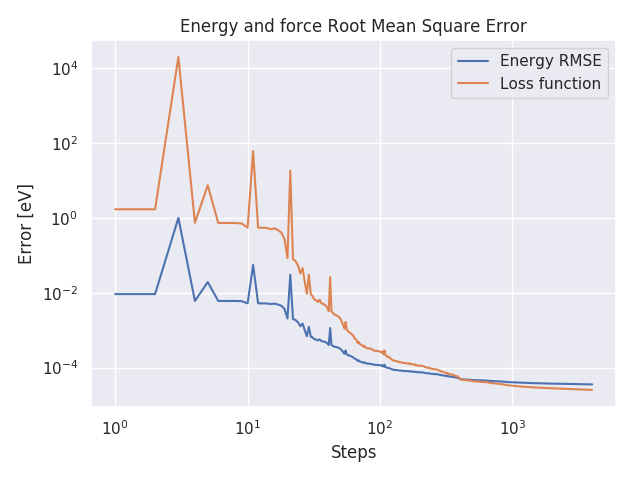
\includegraphics[width=\textwidth]{copper_energy_log.png}
      \caption{Training loss and energy RMSE.}
  \end{subfigure}
  \hfill
  \begin{subfigure}[b]{0.55\textwidth}
      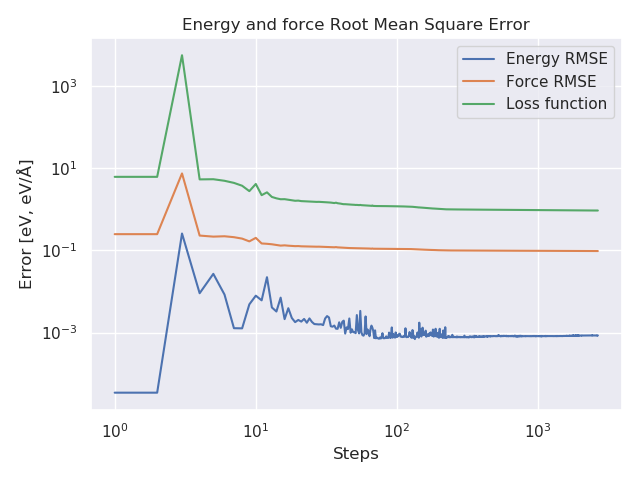
\includegraphics[width=\textwidth]{copper_force_log.png}
      \caption{Training loss and energy and force RMSE.}
  \end{subfigure}
\end{adjustbox}
\end{figure}

In figure \ref{fig:copper-log} we have plotted the loss and root mean
squared errors for the training process.
After a few large oscillations in the beginning
the losses generally settle down and begin to decrease
more smoothly.
After approximately 500-1000 steps the network seems to have
converged, and the change in loss is much smaller than before.
Subsequently we train with forces and we observe a large increase
in the energy RMSE in exchange for a modest decrease in force RMSE,
as discussed in the previous chapter.
After training for a while both errors stop improving,
and we consider the training converged.
Note that the loss function is not equivalent to the energy or force
root mean squared errors, as discussed in chapter \ref{chap:amp-theory}.

\begin{figure}[H]
\begin{adjustbox}{max width=1.2\linewidth,center}
\centering
  \begin{subfigure}[b]{0.55\textwidth}
      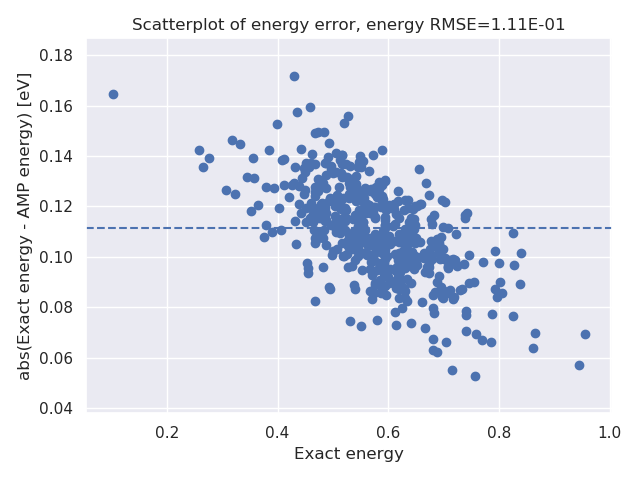
\includegraphics[width=\textwidth]{copper_energy_error.png}
      \caption{Energy error.}
  \end{subfigure}
  \hfill
  \begin{subfigure}[b]{0.55\textwidth}
      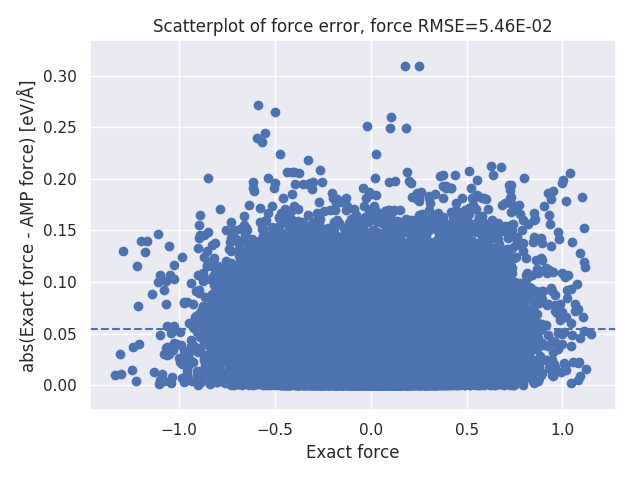
\includegraphics[width=\textwidth]{copper_force_error.png}
      \caption{Force component error.}
  \end{subfigure}
\end{adjustbox}
    \caption{Energy and force component errors on the test images.
        Root mean squared errors in dotted lines.
        The errors are measured in units of eV and eV/Å respectively.}
    \label{fig:copper_error}
\end{figure}

In figure \ref{fig:copper_error} we have plotted the energy and force component
(i.e. in the x,y,z direction)
absolute errors on the EMT test trajectory. We obtain an energy error
of approximately 0.1 eV, with a max value of approximately 0.16 eV.
For the force errors we obtain an force RMSE of 0.05 eV/Å,
but some of the force errors considerably higher, up to
and including values of 0.3 eV/Å, which may pose
a problem for the long term stability of the system.
These values are comparable to other works studying neural network
potential energy surfaces, such as \cite{stende2017constructing,
treider2017speeding, khorshidi2016amp, PhysRevLett.120.143001},
at least for the forces. For the energy, the energy is higher than usual, and
this is caused at least partially by training with force terms.
Generally we observe that large force residuals cause an increase
in energy and translational momentum over time. As we discussed
in chapter \ref{chap:symmetry-functions} we believe this is because
the sampling has left holes in the neural network.

\begin{figure}[H]
    \centering
    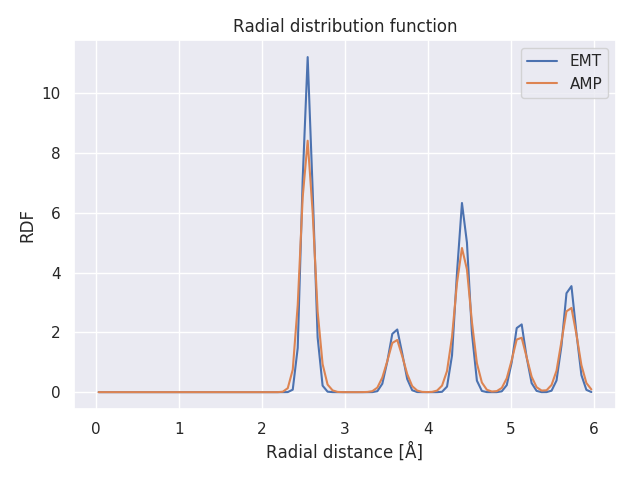
\includegraphics[width=\textwidth]{copper_rdf.png}
    \caption{AMP radial distribution function plotted against
        EMT radial distribution.
        The radial distribution function of the neural network potential is
        generally more dispersed due to the increase in kinetic energy.
        The $y$-axis is the radial distribution function, which is dimensionless.}
    \label{fig:copper-rdf}
\end{figure}

In figure \ref{fig:copper-rdf} we have plotted the AMP neural network
radial distribution function compared to the EMT radial distribution.
We see that the AMP potential can reproduce the copper crystal
structure fairly well, though with smaller peaks.
As we will soon discuss, the neural network appears
to be able to reproduce the equilibrium crystal structure,
though increases in kinetic energy and translational momentum over time
makes the atoms more dispersed.

\begin{figure}[H]
    \centering
    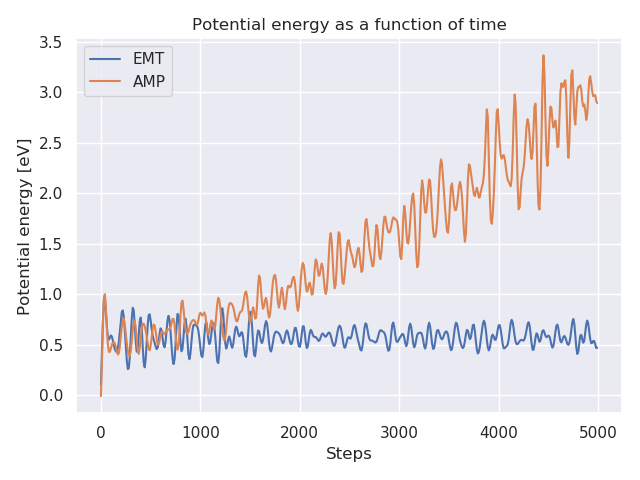
\includegraphics[width=\textwidth]{copper_pot.png}
    \caption{AMP and EMT potential energy as a function of time.
        The potential energy of the neural network generally performs well
        for the first 1000 steps, and then starts to increase
        likely due to an increase in kinetic energy and total energy.}
    \label{fig:copper-pot}
\end{figure}

If we examine the potential energy as a function of time
in figure \ref{fig:copper-pot} we see that the neural network
follows the EMT potential energy fairly well for approximately
1500 steps, but then starts to significantly increase.
As the atoms move away from the energy minimum due to an increase
in kinetic energy, the potential energy starts to increase.
This is most noticeable in figure \ref{fig:copper-energy},
where we have plotted the total energy as a function of time.
While the EMT energy is flat or oscillating around a mean value,
the neural network potential exhibits increasing energy over time.
At the beginning the increase in energy appears to be attributable
to an increase in kinetic energy, which may be caused by errors
in the interpolated forces from the neural network.
This increase in kinetic energy also appears to lead to an increase
in translational momentum.

\begin{figure}[H]
    \centering
    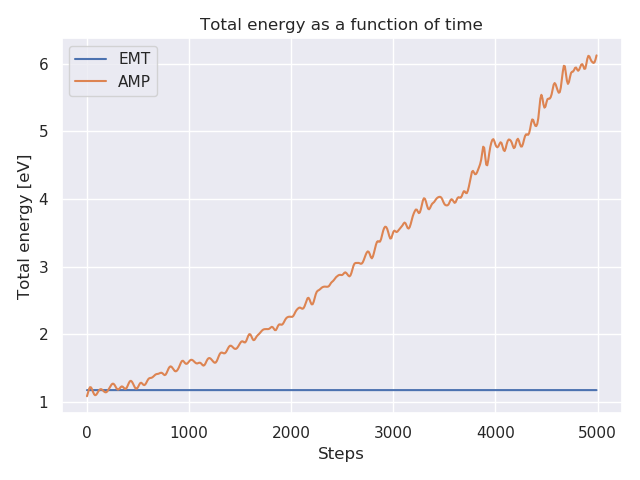
\includegraphics[width=\textwidth]{copper_energy.png}
    \caption{AMP and EMT total energy as a function of time.
    The energy starts increasing after approximately 500 steps,
    and the increase seems to be non-linear. This is hypothesized
    to be due to large force error residuals causing increases in
    the kinetic energy of the atoms.}
    \label{fig:copper-energy}
\end{figure}

In figure \ref{fig:copper-msd} we have plotted the mean squared
displacement (MSD), 
which measures mean distance travelled averaged over all atoms in the system.
We observe that the MSD for the neural network is significantly larger
than for the EMT potential, and increasing non-linearly.
In equilibrium we expect for a crystal lattice
that the mean squared displacement be linear, as the atoms
mostly oscillate in stable energy minima.
For the neural network potential the motion in the system appears
to be increasing significantly, as the kinetic and total energy is increasing
over time.

\begin{figure}[H]
    \centering
    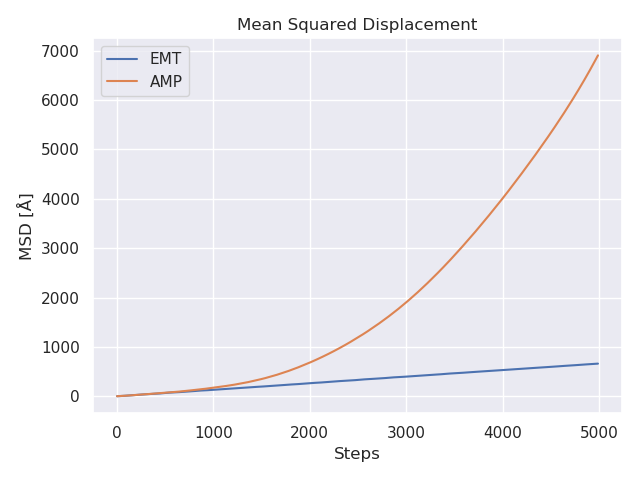
\includegraphics[width=\textwidth]{copper_msd.png}
    \caption{AMP and EMT mean squared displacements as a function of time.
        For the neural network potential the system picks up energy
        and momentum over time, while the atoms governed by the EMT
        potential mostly oscillate in stable energy minima.}
    \label{fig:copper-msd}
\end{figure}

If we examine the system trajectory in a program such as Ovito\footnote{
    \href{https://www.ovito.org/}{Open VIsualization TOol (OVITO)}}
we find that the crystal structure has mostly remained intact, while the
system has picked up a certain amount of translational momentum.
In figure \ref{fig:copper_sw} we see that the system has moved as a whole,
although this is easier to see if you open up the trajectory file in Ovito
yourself.
This is in contrast to the EMT potential, in which the atoms vibrate in place,
and the system remains more or less in place.
Altogether, this suggests that while the neural network potential
is able to reproduce the crystal structure, numerical errors propagate
to a linear (possibly non-linear)
increase in energy over time, which threatens the long-term numerical
stability of the trajectory. In order to obtain better results we would likely
require datasets containing more unlikely configurations and forces
(i.e. slightly out of equilibrium). We also generally find that the performance
improves as we add more symmetry functions, particularly radial functions
are believed to improve the accuracy with this potential,
as the potential contains no explicit treatment of angular interactions.
However, more symmetry functions add significant CPU-time cost,
and the set of symmetry functions would have to be pruned
to remove significant correlations.

\begin{figure}[H]
\begin{adjustbox}{max width=1.2\linewidth,center}
\centering
  \begin{subfigure}[b]{0.55\textwidth}
      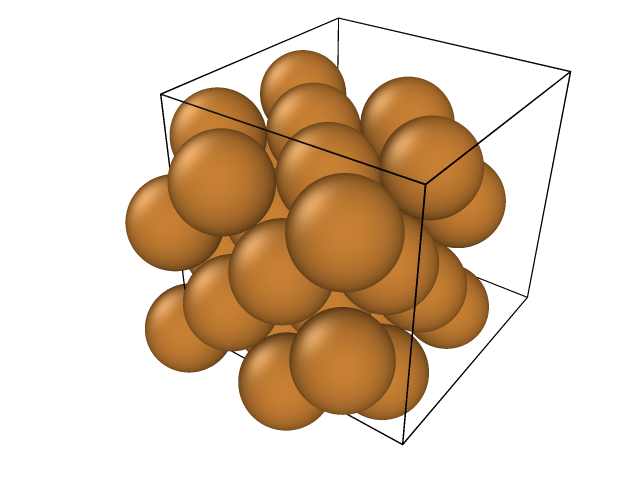
\includegraphics[width=\textwidth]{copper_t0.png}
      \caption{Copper atoms after 10 steps.}
  \end{subfigure}
  \hfill
  \begin{subfigure}[b]{0.55\textwidth}
      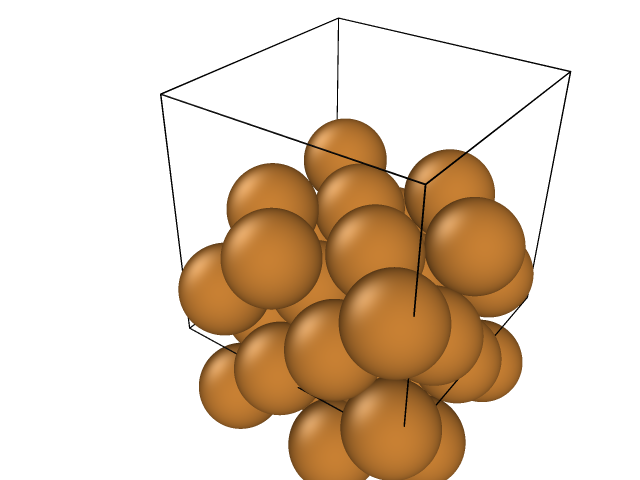
\includegraphics[width=\textwidth]{copper_tn.png}
      \caption{Copper atoms after 5000 steps.}
  \end{subfigure}
\end{adjustbox}
    \caption{The system of copper atoms governed by the neural network
    potential after 10 and 5000 timesteps.
    The system has picked up kinetic energy and momentum and is moving
    over time.}
    \label{fig:copper_sw}
\end{figure}

Finally, we tested the time-scaling of the neural network as the number of atoms
increased. To test this we simply made a forces call on lattices of different
sizes, in order to obtain the force on every atom in the system.
Ideally we would have taken averages over multiple force calls, however
at these time scales we did not think it would significantly impact the results.

\begin{figure}
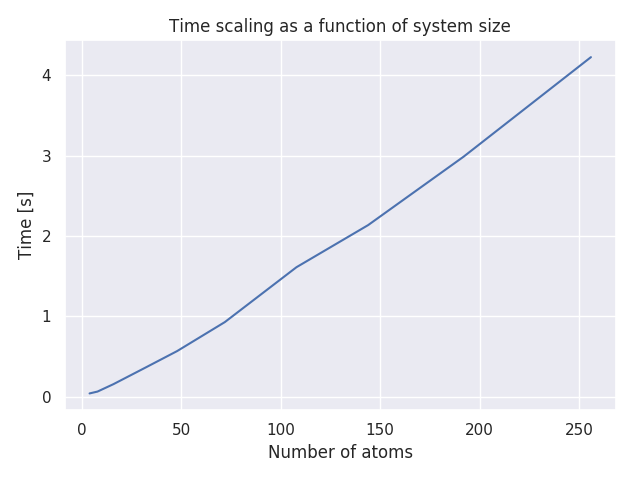
\includegraphics[width=\textwidth]{copper_scaling.png}
\caption{Time scaling of the neural network as the number of atoms increases.
    The time scaling is measured using the time it takes to obtain
    the forces on every atom in the system. The time it takes to obtain
    the forces is generally a linear function of the number of atoms
    in the system.}
\label{fig:copper-scaling}
\end{figure}

In figure \ref{fig:copper-scaling} we see as expected that the 
trained neural network
scales linearly with the number of atoms, though with a significant pre-factor.
We see that it takes approximately 50 seconds to evaluate all the forces
for a system of 50 atoms, while it takes 250 seconds for a system of 200 atoms.
This pre-factor is dependent on the average number of neighbors
of each atom, which is again dependent on the cutoff radius.
Since the neural network has been trained with a set cutoff radius,
this radius should be considered a part of the neural network architecture
and cannot be significantly changed without impacting accuracy.
This pre-factor is of course also dependent on the time it takes to evaluate
the symmetry functions and derivatives, which is dependent on the number
and type of symmetry functions, as the angular function derivatives are significantly
more expensive to evaluate than the radial angular functions.
For the system of 250 atoms the 5000 steps take approximately 2 weeks
to integrate over, which cannot compete with classical potentials,
often evaluated on the order of milliseconds.
However, this is only on a single core, 
and parallelizing using neighbor list algorithms
such as those found in the LAMMPS package 
could be a big improvement without too much overhead.
While this would help deployment, training would still be too slow.
As it stands now, the symmetry function derivatives have significant parts
implemented in Python which could with some effort be moved entirely to Fortran,
such as if-tests, dictionaries and neighbor lists.
If these parts of the codebase were moved fully to a lower-level compiled
language, this would help both training and deployment, and would enable
training and testing of larger and more complex systems\footnote{
    See for example this exchange on the \href{
    https://listserv.brown.edu/cgi-bin/wa?A2=AMP-USERS;d7c6c98c.1904}{
    AMP mailing list}.}.

\subsection{Stillinger-Weber}\label{chap:sw}
The Stillinger-Weber is a potential which describes accurately
Silicon atoms in the diamond lattice structure, and was
one of the first potentials used to describe a realistic atomic-scale
model of Silicon. It is also one of the most common examples
of a potential with a three-body interaction, and its intermediate complexity
makes it ideal for verification with for example quantum calculations
or in our case machine learning methods.
We initialize a system of 8 unit cells with 8 atoms in each unit cell
for a total of $8 \times 2^3 = 64$ atoms with velocities corresponding
to a temperature of 500 Kelvin.
As in the previous section we integrate the system over $9 \cdot 10^5$
steps using a timestep of $\Delta t = 5.0$ fs (suitable for most metals
in a crystalline structure) writing to file every 100 steps
for a total of 8000 images for energy learning
and 1000 images used to train forces.
The neural network is trained for 4000 steps after using simulated annealing
for 2000 steps in order to search for optimal initial weights.
We then generate test sets using the Stillinger-Weber and trained neural network
potentials integrated for 5000 steps and compare the results 
using the potential energy, radial distribution function, 
mean squared displacement and more.
The cutoff radius is set to $R_c = 5$ Angstrom using 14 radial and
22 angular symmetry functions of the G2 and G4 types.

\begin{figure}[H]
\begin{adjustbox}{max width=1.2\linewidth,center}
\centering
  \begin{subfigure}[b]{0.55\textwidth}
      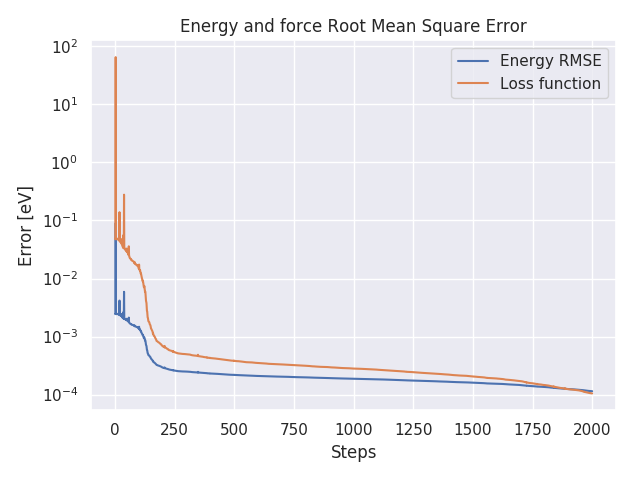
\includegraphics[width=\textwidth]{silicon_energy_log.png}
    \caption{Training loss and energy RMSE.}
  \end{subfigure}
  \hfill
  \begin{subfigure}[b]{0.55\textwidth}
      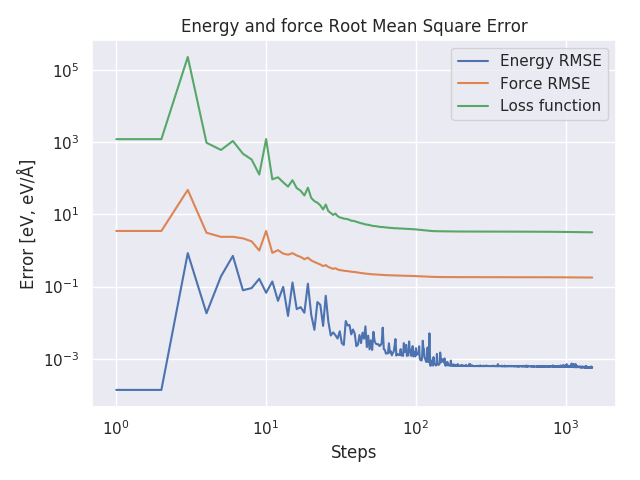
\includegraphics[width=\textwidth]{silicon_force_log.png}
    \caption{Training loss and energy and force RMSE.}
  \end{subfigure}
\end{adjustbox}
\caption{Training losses and energy and force root mean squared errors.
    The loss function is discussed in chapter \ref{chap:amp-theory}.
    The network is first trained only with energies, and subsequently
    using both energies and forces.
    The neural network weight updates are generally small after approximately
    1000 epochs.}
    \label{fig:silicon-log}
\end{figure}

For both the energy training and the force training phases, the 
losses often rise sharply at the beginning, and then decay smoothly over time,
reaching something of a convergence after approximately 500-1000 steps.
These values are somewhat comparable to other works studying neural network
potential energy surfaces, such as \cite{stende2017constructing,
treider2017speeding, khorshidi2016amp, PhysRevLett.120.143001},
at least in terms of the forces, though the energies are higher than usual.
The losses are somewhat higher for the Stillinger-Weber than for the
EMT potential, this may indicate more difficulty reproducing the distribution
or overfitting for the EMT potential.
This is also indicated in the test losses in figure \ref{fig:silicon-error},
where both the energy and force RMSEs are slightly higher than for the
EMT potential. This may also be an artifact of initialization, as finding
good high-dimensional minima using gradient descent 
is a process which in some cases may require many restarts.
However, if we examine the energies interpolated over time,
it paints a better picture than for the EMT potential.

\begin{figure}[H]
\begin{adjustbox}{max width=1.2\linewidth,center}
\centering
  \begin{subfigure}[b]{0.55\textwidth}
      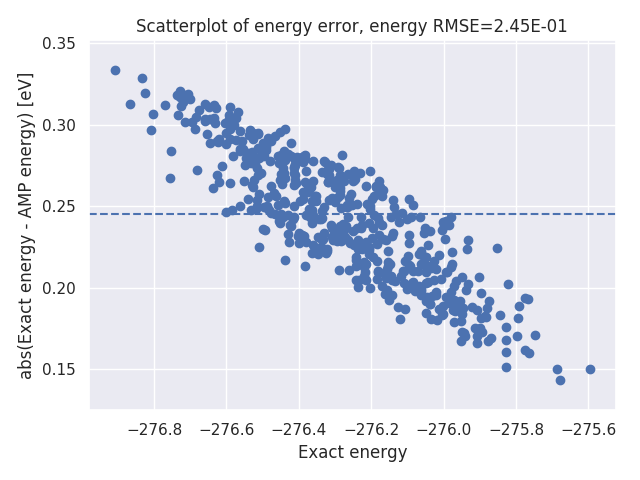
\includegraphics[width=\textwidth]{silicon_energy_error.png}
      \caption{Energy error.}
  \end{subfigure}
  \hfill
  \begin{subfigure}[b]{0.55\textwidth}
      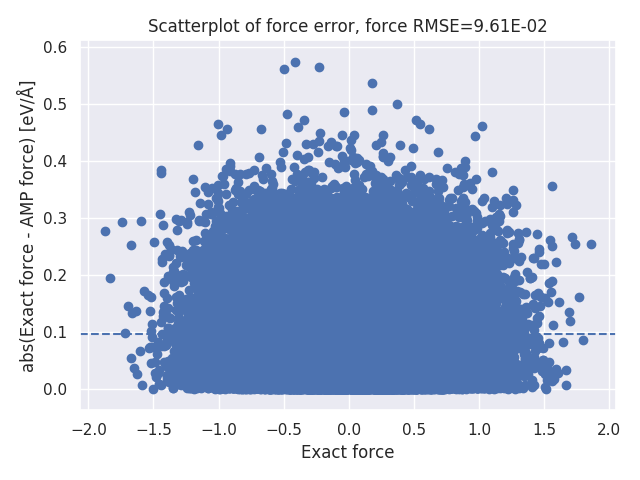
\includegraphics[width=\textwidth]{silicon_force_error.png}
      \caption{Force component error.}
  \end{subfigure}
\end{adjustbox}
    \caption{Energy and force component errors on test trajectory.
        Root mean squared errors in dotted lines.
        The errors are measured in units of eV and eV/Å respectively.}
    \label{fig:silicon-error}
\end{figure}

In figure \ref{fig:silicon-energy} we have plotted the energy as a function
of time. While the energy for the Stillinger-Weber potential 
is flat or oscillating around a mean value over time,
the neural network exhibits as before a seemingly
linear increase in energy over time.
However, if we compare with the EMT potential the change over time 
is now significantly smaller.

\begin{figure}[H]
    \centering
    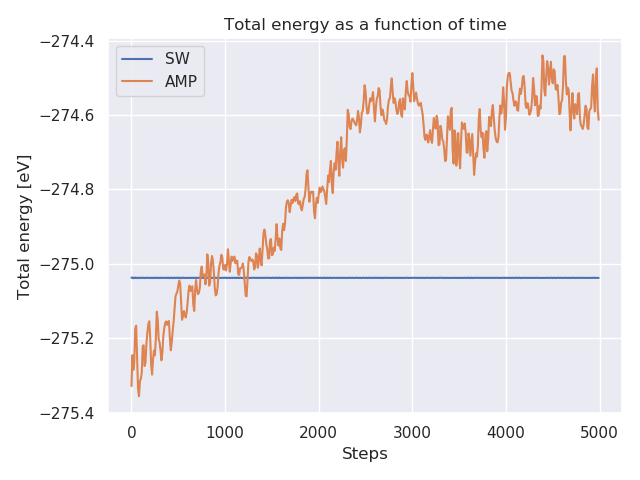
\includegraphics[width=\textwidth]{silicon_energy.png}
    \caption{AMP and Stillinger-Weber total energy as a function of time.
        The energy conservation is generally much better for the
        neural network trained on the Stillinger-Weber potential
        than the one trained on the EMT potential.
        The energy is increasing over time, but may have
        stabilized after approximately 2500 steps. Longer trajectories
        would have to be produced in order to verify this.}
    \label{fig:silicon-energy}
\end{figure}

This is also seen in the potential energy over time 
in figure \ref{fig:silicon-pot}, which is as before increasing,
though the increase is smaller, and in general the potential energy 
fits better than before.
We speculate on a few reasons for this.
One reason may be that since angular interactions contribute significantly to the
Stillinger-Weber potential, a mix of radial and angular symmetry functions
provides a better fit than for the EMT potential, where only radial interactions
are explicitly treated.
Another reason may also be that the Silicon atoms are radially distributed
more discretely, such that there are fewer neighbors for any given
atom to consider.
We expect in general that if the symmetry functions are not too correlated,
adding more symmetry functions increase fit and numerical stability, but
we are limited by the time it takes to evaluate their derivatives.

\begin{figure}[H]
    \centering
    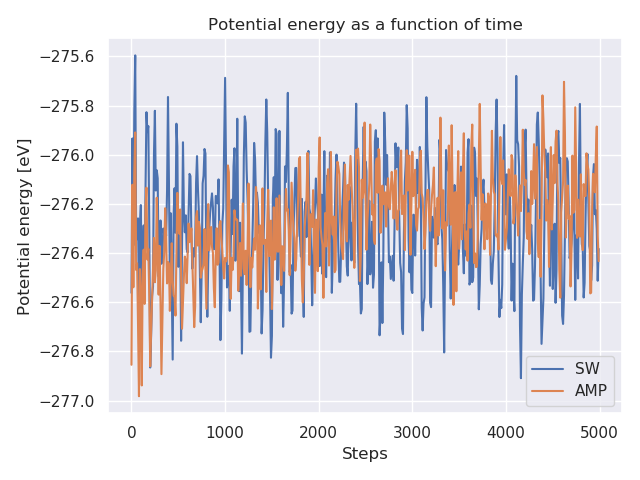
\includegraphics[width=\textwidth]{silicon_pot.png}
    \caption{AMP and Stillinger-Weber potential energy as a function of time.
    The neural network is able to reproduce the Stillinger-Weber potential
    well, but appears to be increasing slightly over time.}
    \label{fig:silicon-pot}
\end{figure}

As before there are indications that the increase in energy 
is initially attributed to the kinetic energy,
and as we see in the radial distribution functions in figure 
\ref{fig:silicon-rdf}, the neural network
system is slightly more dispersed than the Stillinger-Weber system.
In addition in figure \ref{fig:silicon-msd} we can see that the mean squared
displacement is increasing in a non-linear fashion as the atoms pick up
both kinetic energy and translational momentum.

\begin{figure}[H]
    \centering
    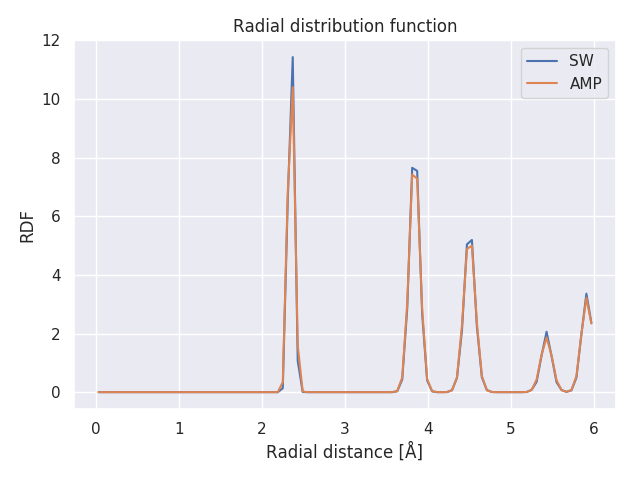
\includegraphics[width=\textwidth]{silicon_rdf.png}
    \caption{Radial distribution functions for the Stillinger-Weber and
        neural network potentials.
        The system governed by the neural network potential is more dispersed
        over time, due to an increase in kinetic and total energy.}
    \label{fig:silicon-rdf}
\end{figure}

The increase in kinetic energy and translational momentum is illustrated
both in the mean squared displacement and from snapshots of the system
as in figure \ref{fig:silicon-time}. This is even better illustrated
in visualization software, where we can see that while the
Stillinger-Weber system remains stationary over time, the neural network
system picks up momentum and starts moving.
We see that the system has moved slightly over time, while the crystal
structure has remained mostly intact as evidenced by the radial distribution
function.
However, since the energy conservation is better for the neural network
trained on the Stillinger-Weber potential, this motion is smaller
than what we have observed for the EMT potential.

\begin{figure}[H]
    \centering
    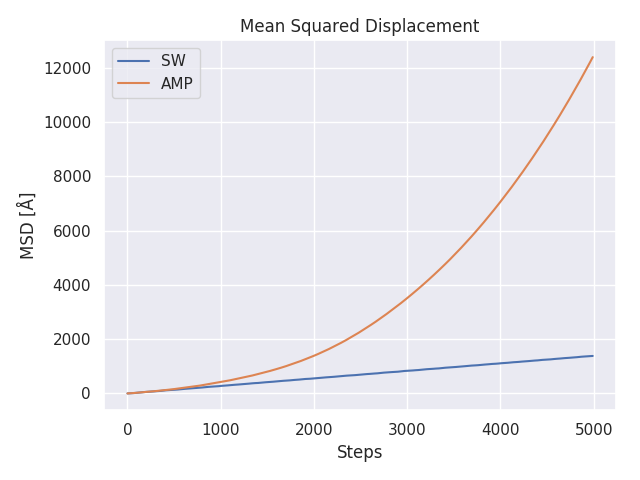
\includegraphics[width=\textwidth]{silicon_msd.png}
    \caption{Mean squared displacement over time for the Stillinger-Weber
        and neural network potentials.
        For the neural network potential the system picks up some energy
        and momentum over time, while the atoms governed by the Stillinger-Weber
        potential mostly oscillate in stable energy minima.}
    \label{fig:silicon-msd}
\end{figure}

\begin{figure}[H]
\begin{adjustbox}{max width=1.2\linewidth,center}
\centering
  \begin{subfigure}[b]{0.55\textwidth}
      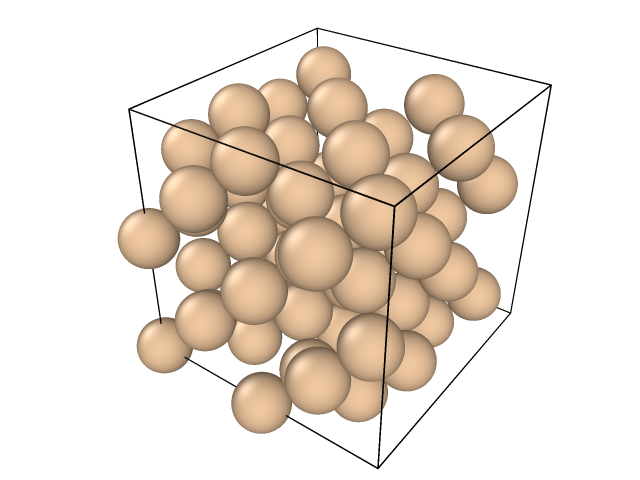
\includegraphics[width=\textwidth]{silicon_t0.png}
      \caption{Silicon atoms after 10 steps.}
  \end{subfigure}
  \hfill
  \begin{subfigure}[b]{0.55\textwidth}
      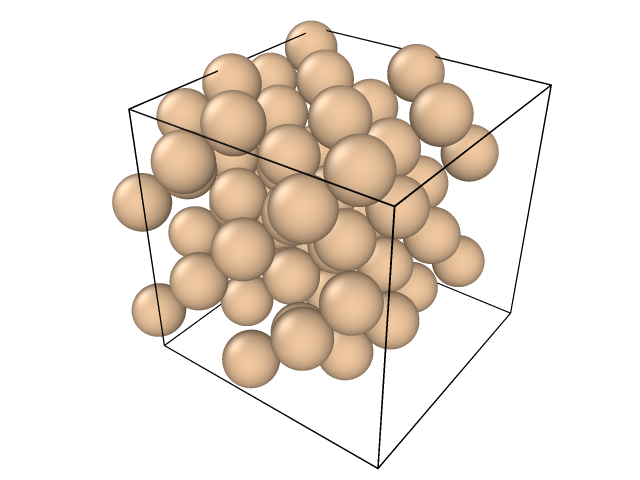
\includegraphics[width=\textwidth]{silicon_tn.png}
      \caption{Silicon atoms after 5000 steps.}
  \end{subfigure}
\end{adjustbox}
    \caption{The system of silicon atoms governed by the neural
    network potential after 10 and 5000 steps.
    The system has picked up some kinetic energy and momentum and is moving
    over time.}
    \label{fig:silicon-time}
\end{figure}

Finally, we also examined the time scaling of the system as we did for the
neural network trained on the EMT potential.
As before we calculated the time it took for a single forces call
on all the atoms in the system, as this is the limiting
factor for integrating the atoms a single timestep using the
Verlet algorithm.
Ideally we would take averages of the time this takes, but except
for the smaller systems this does not affect the results very much,
due to the timescales involved.
The results are shown in figure \ref{fig:silicon-scaling}.
From this plot we observe that integrating a system
with 100 silicon atoms one step would take approximately
25-30 seconds, while a system of 300 atoms would take approximately
110 seconds. This means integrating a system of 100 atoms
for 5000 steps would take about 35 hours, which is quite
a large amount of time compared to typical empirical potentials.
For the Stillinger-Weber potential this force call
takes on the order of milliseconds, several orders of magnitude removed.
However, since the neural network potential scales linearly, this may be competive
with ab-initio methods which exhibit much poorer scaling as the system size increases.

\begin{figure}
    \centering
    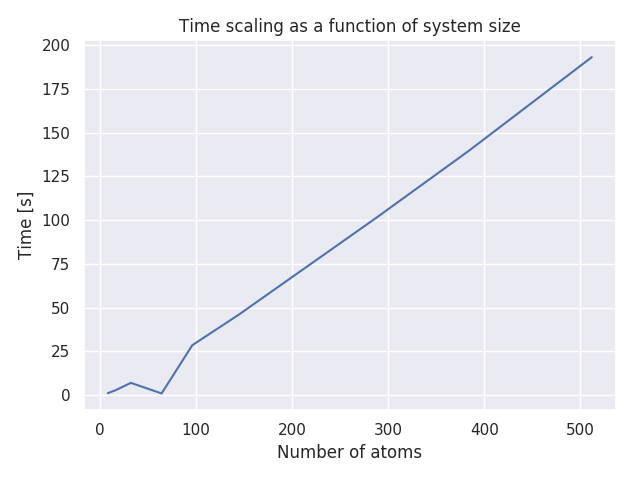
\includegraphics[width=\textwidth]{silicon_scaling.png}
    \caption{Time scaling of the neural network potential
        as a function of the size of the system.
    The time scaling is measured using the time it takes to obtain
    the forces on every atom in the system. The time it takes to obtain
    the forces is generally a linear function of the number of atoms
    in the system.}
    \label{fig:silicon-scaling}
\end{figure}

Even though the neural network potentials have the same cutoff radius,
the Stillinger-Weber potential takes roughly 2-4 times fewer seconds to evaluate
the forces for an equivalent size. It is unclear why this is the case,
as the trained potentials have a comparable number of radial symmetry functions,
while the Stillinger-Weber potential has a larger amount of angular symmetry 
functions.
This may be because the copper atoms have a larger average amount of neighbors,
or because the potentials have been tested on different computers (due to some
    difficulty in installing the Stillinger-Weber potential on one computer).
Otherwise, this may be down to bugs in the code which stalls the network
when calculating neighborlists, fingerprints or other quantities.
